\documentclass[conference]{IEEEtran}
\IEEEoverridecommandlockouts
\usepackage{cite}
\usepackage{amsmath,amssymb,amsfonts}
\usepackage{graphicx}
\usepackage{textcomp}
\usepackage{xcolor}
\usepackage{booktabs}
\usepackage{multirow}
\usepackage{url}

\begin{document}

\title{Reproducible Synthetic Denoising: A PhD Lab QA Experiment}

\author{\IEEEauthorblockN{QA Fixture}
\IEEEauthorblockA{}}

\maketitle

\begin{abstract}
This technical report validates a synthetic CPU workflow, not a new empirical scientific result.
\end{abstract}

\begin{IEEEkeywords}
synthetic data, denoising, reproducibility, quality assurance
\end{IEEEkeywords}

% ===== methodology =====
\section{Methodology}
We use 128 sine samples with Gaussian noise sigma 0.25 and a three-point moving average. The authored fixture is cited as \cite{fixturendsynthetic}.

% ===== experiments =====
\section{Experiments and Results}
The measured noisy MSE is 0.052396280822; filtered MSE is 0.018616959299. Fresh subprocess replay and independent recomputation agree within $10^{-12}$.
\begin{figure}[h]\centering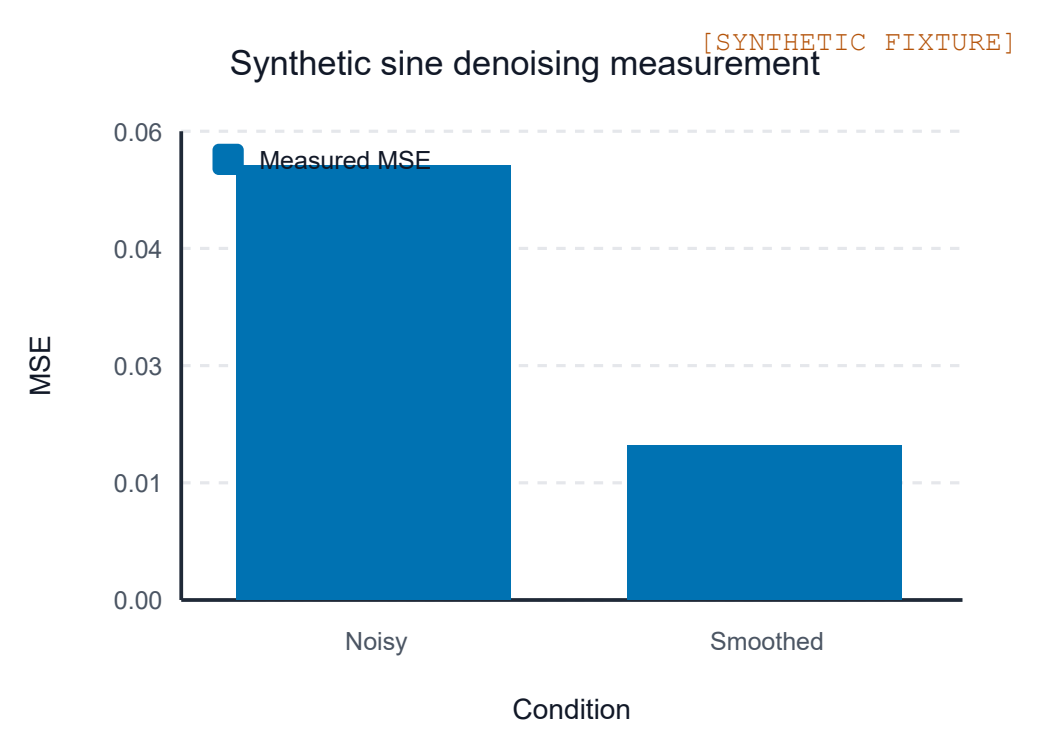
\includegraphics[width=0.7\linewidth]{figure.png}\caption{Measured MSE on the synthetic CPU fixture.}\end{figure}

% ===== discussion =====
\section{Discussion}
The dataset is synthetic. No generalization, novelty, provider parity or peer-review approval is claimed.

\bibliographystyle{IEEEtran}
\bibliography{references}

\end{document}
